\clearpage
\VerdierPhysicalPageAnchor{0237}%
\begingroup\small\setlength{\parskip}{0pt}\setlength{\emergencystretch}{1.5em}
\setlength{\abovedisplayskip}{4pt plus 2pt minus 2pt}%
\setlength{\belowdisplayskip}{4pt plus 2pt minus 2pt}%

\VerdierSemanticAnchor{ch4d-4-3-2}
\noindent\textbf{Proposition 4.3.2.}\quad
\textit{Soient $X$ un objet de $\operatorname{comp}(\mathcal A)$,
$\bigl(X(p,q),\delta(p,q,r)\bigr)$ le deuxième objet spectral associé à
$X$ et $H\colon D(\mathcal A)\longrightarrow\mathcal A$ le foncteur
cohomologique canonique.}

\VerdierSemanticAnchor{ch4d-4-3-2-a}
\noindent\textit{a) $H^r\bigl(X(p,q)\bigr)=0$, pour tout entier $r<p$ ou
$r\geq q$.}

\VerdierSemanticAnchor{ch4d-4-3-2-b}
\noindent\textit{b) Soit $r$ un entier. Pour tout élément $(p,q)$ de
$\mathcal{F}\ell_1(\widetilde{\mathbb Z})$ tel que $p\leq r<q$, il existe
un et un seul isomorphisme :}
\[
i_{p,q}^r(X)\colon H^r(X)\xrightarrow{\sim}H^r\bigl(X(p,q)\bigr)
\]
\noindent\textit{tel que $i_{-\infty,+\infty}^r(X)$ soit l'identité et tel
que pour tout couple $(p,q)$ et $(p',q')$, $p\leq p'$, $q\leq q'$,
$p\leq r<q$, $p'\leq r<q'$, le diagramme ci-après soit commutatif :}

\VerdierSemanticAnchor{ch4d-4-3-2-b-diagram}
\begin{center}
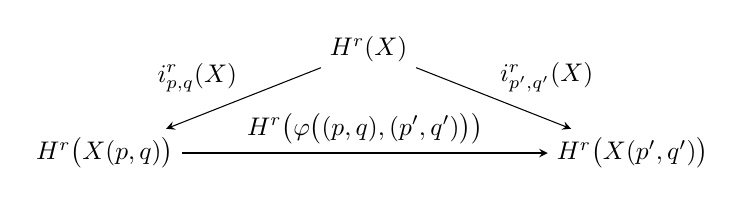
\begin{tikzpicture}[>=stealth,line width=.38pt,x=2.35cm,y=1.15cm,
  scale=.92,transform shape]
  \node (HX)  at (1.55,1.25) {$H^r(X)$};
  \node (Hpq) at (0,0) {$H^r\bigl(X(p,q)\bigr)$};
  \node (Hpp) at (3.10,0) {$H^r\bigl(X(p',q')\bigr)$};
  \draw[->] (HX) -- node[above left=-1pt] {$i_{p,q}^r(X)$} (Hpq);
  \draw[->] (HX) -- node[above right=-1pt] {$i_{p',q'}^r(X)$} (Hpp);
  \draw[->] (Hpq) -- node[above]
    {$H^r\!\left(\varphi\bigl((p,q),(p',q')\bigr)\right)$} (Hpp);
\end{tikzpicture}
\end{center}

\VerdierSemanticAnchor{ch4d-4-3-2-c}
\noindent\textit{c) Soient $m\colon X\longrightarrow Y$ un morphisme de
$\operatorname{comp}(\mathcal A)$ et :}
\[
m(p,q)\colon X(p,q)\longrightarrow Y(p,q)
\]
\noindent\textit{le morphisme correspondant entre les deuxièmes objets
spectraux associés. Pour tout élément $(p,q)$ de
$\mathcal{F}\ell_1(\widetilde{\mathbb Z})$ et tout entier $r$ tel que
$p\leq r<q$, le diagramme ci-après est commutatif :}

\VerdierSemanticAnchor{ch4d-4-3-2-c-diagram}
\begin{center}
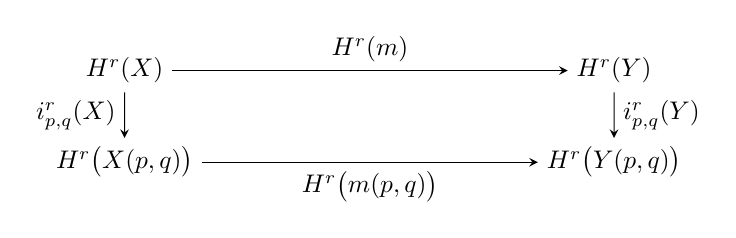
\begin{tikzpicture}[>=stealth,line width=.38pt,x=2.55cm,y=1.10cm,
  scale=.92,transform shape]
  \node (HX)  at (0,1.15) {$H^r(X)$};
  \node (HY)  at (2.65,1.15) {$H^r(Y)$};
  \node (Hpq) at (0,0) {$H^r\bigl(X(p,q)\bigr)$};
  \node (HpY) at (2.65,0) {$H^r\bigl(Y(p,q)\bigr)$};
  \draw[->] (HX) -- node[above] {$H^r(m)$} (HY);
  \draw[->] (Hpq) -- node[below] {$H^r\bigl(m(p,q)\bigr)$} (HpY);
  \draw[->] (HX) -- node[left] {$i_{p,q}^r(X)$} (Hpq);
  \draw[->] (HY) -- node[right] {$i_{p,q}^r(Y)$} (HpY);
\end{tikzpicture}
\end{center}

\noindent Cette proposition résulte immédiatement des définitions.

\VerdierSemanticAnchor{ch4d-4-3-3}
\medskip\noindent\textbf{Corollaire 4.3.3.}\quad
\textit{Le foncteur deuxième objet spectral canonique (4.3.1) se factorise
d'une manière unique à travers le foncteur canonique :}
\[
\operatorname{comp}(\mathcal A)\longrightarrow D(\mathcal A).
\]

\VerdierSemanticAnchor{ch4d-4-3-3-proof}
En effet, d'après (4.3.2), un quasi-isomorphisme
$m\colon X\longrightarrow Y$ est transformé par ce foncteur en isomorphisme
d'objets spectraux. Le corollaire résulte donc de (1.3.5).
\endgroup
